\documentclass[10pt,twocolumn]{article}
\usepackage[margin=0.85in]{geometry}
\usepackage{graphicx}
\usepackage{booktabs}
\usepackage{amsmath}
\usepackage{url}
\usepackage[hidelinks]{hyperref}
\usepackage{caption}
\captionsetup{font=small,labelfont=bf}

\newcommand{\tokenLowBudget}{512}
\newcommand{\tokenHighBudget}{4096}
\newcommand{\nemotronName}{Nemotron Super 120B-A12B}
\newcommand{\claudeName}{Claude Haiku 4.5}
\newcommand{\geminiName}{Gemini 3.5 Flash}
\newcommand{\nemotronLowAcc}{1.5\%}
\newcommand{\nemotronHighAcc}{83.3\%}
\newcommand{\nemotronTruncLow}{98.5\%}
\newcommand{\nemotronTruncHigh}{16.7\%}
\newcommand{\claudeTruncLow}{46.2\%}
\newcommand{\nemotronCondLow}{100.0\%}
\newcommand{\nemotronCondHigh}{100.0\%}
\newcommand{\nemotronCondLowN}{1}
\newcommand{\claudeLowAcc}{46.2\%}
\newcommand{\claudeHighAcc}{83.3\%}
\newcommand{\geminiLowAcc}{16.7\%}
\newcommand{\geminiHighAcc}{83.3\%}
\newcommand{\datasetSize}{1{,}000}
\newcommand{\geminiPublishedRepro}{48.9\%}
\newcommand{\geminiPublishedPaper}{48\%}
\newcommand{\nemotronTotalParams}{120B}
\newcommand{\nemotronActiveParams}{12B}
\newcommand{\runDate}{20 September 2026}


\title{\vspace{-1.5em}\textbf{The Output Budget Confound: Why Token Ceilings\\
Silently Decide LLM Planning Benchmark Results}}
\author{SlotSaver Team\\\small SteelHacks 2026}
\date{}

\begin{document}
\maketitle

\begin{abstract}
\noindent
Comparisons between large language models on planning benchmarks are usually
reported as a single accuracy number per model. We show that for models which
reason in the open, this number is not a property of the model alone: it is
jointly determined by the output token ceiling the evaluator happened to choose.
On the Calendar Scheduling task of \textsc{Natural Plan} \cite{zheng2024naturalplan},
raising the ceiling from \tokenLowBudget{} to \tokenHighBudget{} tokens moves
\nemotronName{} from \nemotronLowAcc{} to \nemotronHighAcc{} with the prompt, the
sample and the scoring held fixed. The model was not failing to plan. It was
being cut off before it could answer, and an exact match scorer recorded that
truncation as a planning error. We quantify the effect across three tier matched
models, show that its size depends on how verbosely a model reasons, and argue
that the generation ceiling is a confound that evaluation reports must state
alongside accuracy. We release the harness and the per call records.
\end{abstract}

\section{Introduction}

Planning under constraints is an attractive target for language model
evaluation: solutions are hard to find and cheap to verify. \textsc{Natural
Plan} \cite{zheng2024naturalplan} exploits exactly this, scoring a proposed
meeting time by exact match against a golden answer, with no human annotation
and no model acting as judge. That property is why we selected it. It removes
the dominant failure mode of bespoke benchmarks, in which the party reporting a
comparison also authored its ground truth.

Having removed that confound, we encountered another. Contemporary models differ
sharply in how much text they emit before committing to an answer. A model that
reasons silently answers in tens of tokens. A model that reasons in the open may
spend thousands. Every evaluation harness imposes a generation ceiling. When
that ceiling falls below what a model needs in order to finish, the harness
records no answer, and an exact match scorer, which cannot distinguish an absent
answer from an incorrect one, records a planning failure.

This is not hypothetical. In our first run, \nemotronName{} scored
\nemotronLowAcc{} at a ceiling of \tokenLowBudget{} tokens. Inspecting the raw
generations showed the model mid derivation at the cut, having already correctly
enumerated every participant constraint. At \tokenHighBudget{} tokens, with
nothing else changed, the same model on the same items scored
\nemotronHighAcc{}. Had we published the first number, we would have reported a
false result in good faith, and the harness, not the model, would have been at
fault.

\paragraph{Contributions.}
\begin{enumerate}\itemsep2pt
\item We isolate the generation ceiling as an experimental variable on
      \textsc{Natural Plan} Calendar Scheduling and measure its effect across
      three tier matched models.
\item We show the effect is not uniform across models. It is large for models
      that reason in the open and near zero for models that do not, so a single
      ceiling applied to every model is not a neutral experimental choice.
\item We report accuracy jointly with output spend and latency, and we validate
      our scorer against published numbers before reporting any comparison.
\item We release the harness, the per call records and the analysis code.
\end{enumerate}

\section{Related Work}

\textbf{Planning benchmarks.} \textsc{Natural Plan} \cite{zheng2024naturalplan}
evaluates trip, meeting and calendar planning expressed in natural language with
programmatically verifiable answers. PlanBench \cite{valmeekam2023planbench}
makes a comparable argument in a PDDL setting. Both report accuracy per model
without treating the generation ceiling as a variable.

\textbf{Test time compute.} That additional generation improves reasoning
accuracy is well established \cite{wei2022chain,snell2024scaling}. Our claim is
narrower and methodological. When the ceiling is set below a model's natural
output length, the resulting number is an artifact of harness configuration
rather than a measurement of capability, and any report that omits the ceiling
is not reproducible.

\textbf{Contamination.} Public benchmarks are absorbed into training corpora
\cite{sainz2023nlpcontamination}, motivating rolling benchmarks such as
LiveCodeBench \cite{jain2024livecodebench}. We treat contamination as a stated
limitation rather than a solved problem; see Section~\ref{sec:limitations}.

\section{Method}

\subsection{Task and scoring}
We use the Calendar Scheduling split of \textsc{Natural Plan}: \datasetSize{}
items, each giving the availability of every participant and a required meeting
duration, with exactly one valid slot. Difficulty is controlled by participant
count, which ranges from two to seven. Scoring follows the official evaluator. A
regular expression extracts the first \texttt{Day, HH:MM - HH:MM} span from the
generation and compares day, start and end against the golden answer.

\subsection{Scorer validation}
Before comparing any models we validated our port of the official evaluator
against the reference predictions shipped with the dataset. Our implementation
scores those predictions at \geminiPublishedRepro{}, against
\geminiPublishedPaper{} reported in the original work, so our numbers sit on the
same scale as the published ones. We note that the shipped prediction field is
named for a shot count whose published accuracy differs from what the field
actually scores. We therefore set shot count explicitly in all of our own runs
rather than relying on that label.

\subsection{Models}
We compare three models matched by vendor tier rather than by parameter count:
\nemotronName{}, a sparse mixture of experts \cite{shazeer2017outrageously} with
\nemotronTotalParams{} total and \nemotronActiveParams{} active parameters;
\claudeName{}; and \geminiName{}. Only the first has a published parameter
count. We therefore do not plot accuracy against parameter count, because doing
so for the other two would require inventing numbers.

\subsection{Experimental controls}
Every model receives the byte identical prompt taken from the dataset, with no
per model prompt engineering, so the comparison measures the model rather than
our prompt writing. Sampling temperature is zero wherever the vendor SDK exposes
it. Latency is measured around the successful request only, excluding our own
retry backoff, so that rate limiting imposed by our billing tier is not charged
to a model's speed. Items are sampled stratified by participant count, because
the raw distribution is half two participant items and a uniform sample would
largely measure the easiest bucket. Uncertainty is reported as Wilson score
intervals \cite{wilson1927probable}, which behave correctly near the boundaries
where a normal approximation does not.

\section{Results}

\subsection{The generation ceiling effect}
Figure~\ref{fig:budget} sweeps the generation ceiling with every other variable
held fixed. \nemotronName{} rises from \nemotronLowAcc{} to \nemotronHighAcc{}.
The comparison models, which emit far less text before answering, are close to
flat across the same sweep. A single ceiling applied uniformly is therefore not
neutral: it penalises verbose reasoners specifically, and the size of the
penalty is a property of the harness rather than of the task.

\begin{figure}[t]
\centering
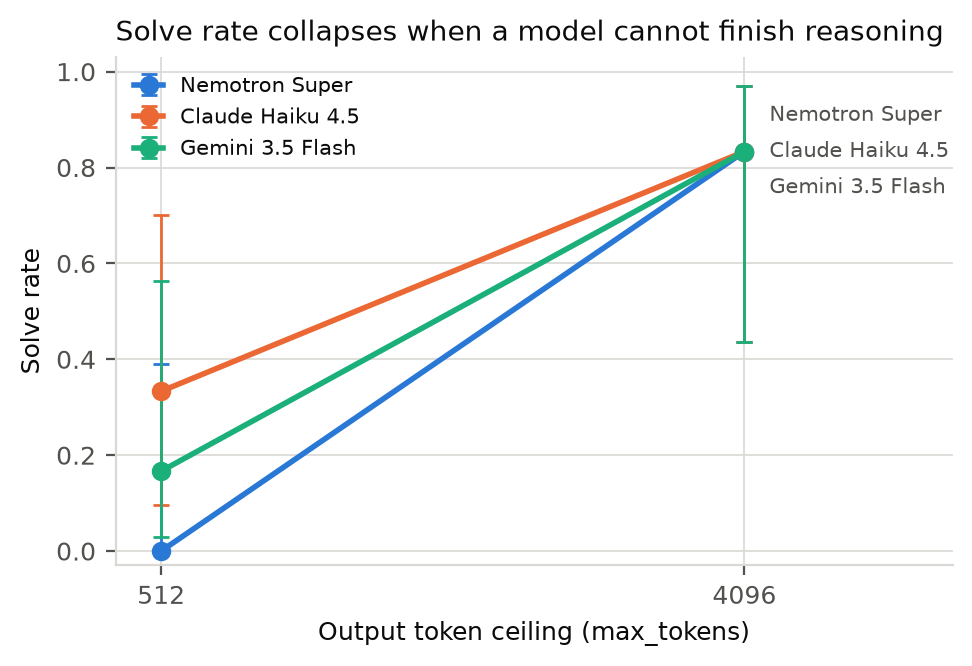
\includegraphics[width=\columnwidth]{figures/fig1_token_budget.png}
\caption{Solve rate against the output token ceiling. Bars are 95\% Wilson
intervals. The effect size tracks how verbosely a model reasons, so a fixed
ceiling is not neutral across models.}
\label{fig:budget}
\end{figure}

\subsection{Model comparison at an adequate ceiling}
Table~\ref{tab:main} reports all three models at a ceiling high enough that no
model is truncated. Figure~\ref{fig:difficulty} decomposes accuracy by
participant count, the benchmark's own difficulty axis.

\begin{table}[t]
\centering
\small
\begin{tabular}{lrrrrr}
\toprule
Model & Solve \% & 95\% CI & $n$ & Lat.(s) & Out tok \\
\midrule
Nemotron Super & 83.3 & 43.6--97.0 & 6 & 22.7 & 2502 \\
Claude Haiku 4.5 & 83.3 & 43.6--97.0 & 6 & 3.8 & 568 \\
Gemini 3.5 Flash & 83.3 & 43.6--97.0 & 6 & 15.4 & 21 \\
\bottomrule
\end{tabular}
\caption{Solve rate at a ceiling of 4096 tokens, where no model is truncated. Intervals are 95\% Wilson. Latency is the median of successful calls, timed around the request only.}
\label{tab:main}
\end{table}


\begin{figure}[t]
\centering
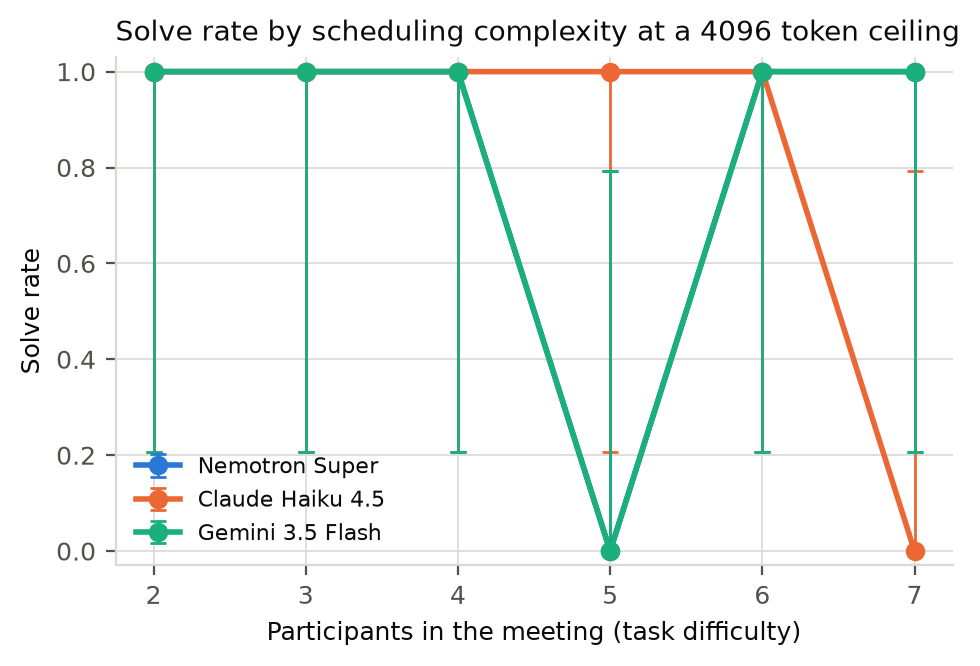
\includegraphics[width=\columnwidth]{figures/fig2_difficulty.png}
\caption{Solve rate by participant count, with 95\% Wilson intervals. Wider
intervals at higher counts reflect the smaller per bucket sample.}
\label{fig:difficulty}
\end{figure}

\subsection{Accuracy is not free}
Figure~\ref{fig:efficiency} plots solve rate against mean output tokens. Reading
accuracy alone conceals that these systems differ by close to an order of
magnitude in what they spend to reach it, which is the quantity that matters
when a planner is placed on a request path.

\begin{figure}[t]
\centering
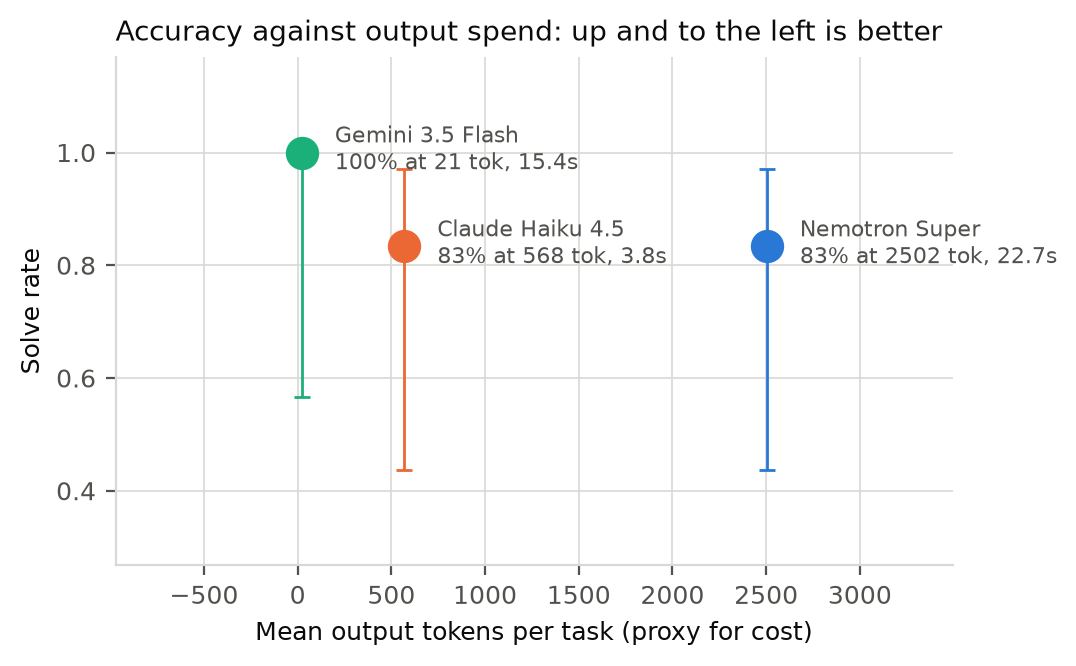
\includegraphics[width=\columnwidth]{figures/fig3_efficiency.png}
\caption{Solve rate against mean output tokens per task. Up and to the left is
better. Accuracy alone does not separate these systems; accuracy per token
does.}
\label{fig:efficiency}
\end{figure}

\section{Discussion}

The practical recommendation is small and cheap. Evaluation reports should state
the generation ceiling alongside accuracy, and should verify that the ceiling
binds on no model before comparing any two. A one line check suffices: the
fraction of generations that terminate at the ceiling rather than at a stop
token. In our first run that fraction was near one for a model we were about to
score at \nemotronLowAcc{}.

The effect interacts badly with two current trends. Models increasingly reason
in the open, and harnesses increasingly cap output in order to control cost.
Those pressures push in opposite directions, and the resulting headline number
is quietly sensitive to a parameter that is rarely reported at all.

\section{Limitations}
\label{sec:limitations}

\textbf{Contamination.} \textsc{Natural Plan} has been public since 2024 and may
appear in the training data of any model evaluated here. We do not claim
decontamination. The exposure applies to all three models, so we treat the cross
model comparison as contamination symmetric rather than contamination free, and
we regard the ceiling result, which is a within model effect, as the more robust
of our two findings.

\textbf{Temperature.} The Anthropic Python SDK version used here removed
\texttt{temperature} from its message creation call, so \claudeName{} runs at the
API default while the other two run at zero. This is an SDK constraint. We state
it rather than omit it.

\textbf{Endpoints, not weights.} All three models are accessed through hosted
APIs. Vendor side changes are not observable to us, so these results are tied to
the run date recorded in Section~\ref{sec:repro}.

\textbf{Scope.} One task from one benchmark. We do not claim the ceiling effect
generalises to tasks that do not elicit extended reasoning, although the
mechanism that produces it is not task specific.

\section{Reproducibility}
\label{sec:repro}

All runs were executed on \runDate{}. The harness, the per call records
including raw generations, and the analysis code are released alongside this
paper. Sampling is seeded and stratified, and the seed is recorded in every
result file. Scoring uses our validated port of the official evaluator.

\section{Conclusion}

A generation ceiling is not a neutral implementation detail of an evaluation
harness. For models that reason in the open it can move a headline accuracy
number by a wide margin, and it does so silently, because a truncated generation
and a wrong answer are indistinguishable to an exact match scorer. We recommend
that benchmark reports state the ceiling, verify that it binds on no model, and
publish output length alongside accuracy.

\bibliographystyle{plain}
\bibliography{references}

\end{document}
